\section{Evaluation}
\label{sect:experiment} 

\subsection{Experiment Setup}
We evaluated QoSManager on a desktop PC with Intel(R) Core(TM) i7-2600 CPU @ 3.40GHz and 8GB RAM. We used Mininet~\cite{mininet} with Open vSwitch~\cite{openvswitch} to emulate
different network scenarios. Mininet uses OS features to instantiate lightweight virtualization of network hosts and interconnects them with virtual switches, according to a
specified topology configuration. Open vSwitch is a software implementation of a virtual multilayer network switch. QoSManager was implemented on top of Ryu~\cite{ryu}, an
open-source SDN controller.

\reffig{setup} shows our experiment setup. There are two switches connected with a 8Mbps link.

\begin{figure}[htb]
\centering
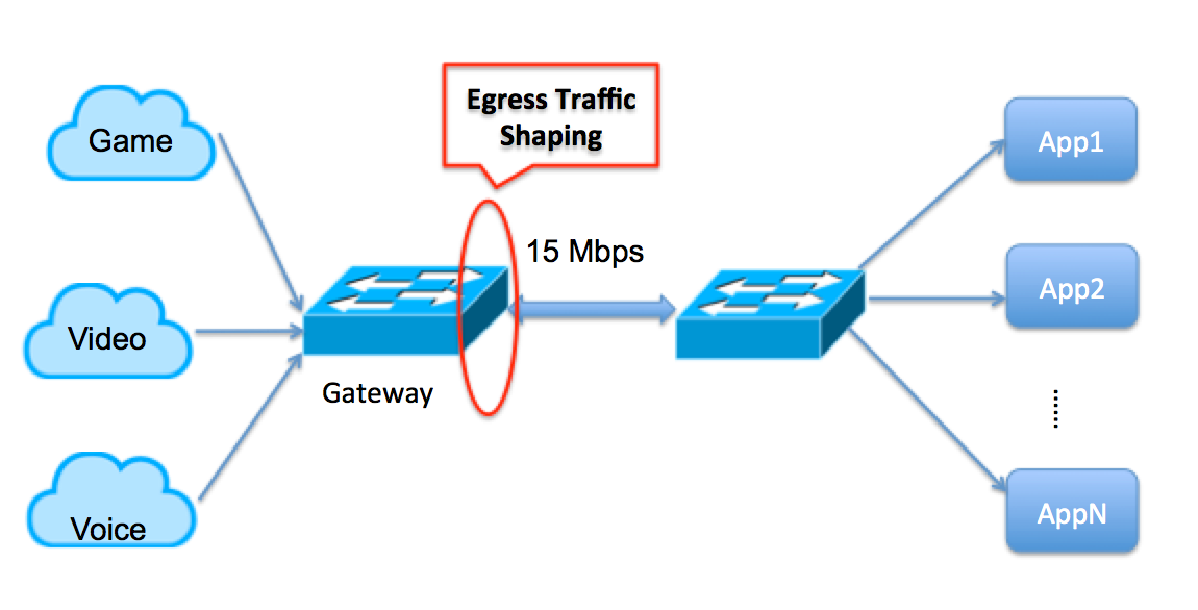
\includegraphics[width=0.5\textwidth]{exp_setup}
\caption{Experiment setup.}
\label{fig:setup}
\end{figure}

During the experiments, different servers send different types of traffic, such as game, video and VoIP, to the clients on the right. All the traffic flows through the link between
the two switches and competes for the scarce bandwidth. The QoS requirements for the services are displayed in~\reftable{qos_config}.

\begin{table}[htb]
\scriptsize
\caption{QoS Configuration}
\begin{tabular}{|l|l|l|l|}
\hline Service type & Minimum bw & Recommended bw & Priority \\
\hline
\hline VoIP & 400Kbps & 1.2Mbps & 10 \\
\hline Video & 3.5Mbps & 5Mbps & 6  \\
\hline Game & 1.7Mbps & 3Mbps & 2  \\
\hline
\end{tabular}
\label{table:qos_config}
\end{table}

We first investigate how QoSManager allocates bandwidth to high priority traffic and low priority traffic. Then, we study whether high priority traffic will be affected by
new low priority flow coming into the network. Finally, we analyze whether high priority traffic can acquire the desired bandwidth in a congested network.

\subsection{Q1: How does QoSManager allocate bandwidth?}

To answer question 1, we created a scenario (scenario 1) where two clients are watching videos while a client is making a VoIP call. The rate of each video stream is 5Mbps, and
the rate of VoIP is 1.2Mbps.

We ran the same scenario twice and compared the bandwidth allocation with and without QoSManger. \reffig{s1_qos} illustrates the bandwidth assigned to the three services with
QoSManager, and \reffig{s1_no_qos} shows the bandwidth assignment without QoSManager. 

\begin{figure}[htb]
\centering
\includegraphics[width=0.32\textwidth,angle=270]{s1_qos}
\caption{Bandwidth allocation in scenario 1 with QoSManager.}
\label{fig:s1_qos}
\end{figure}

\begin{figure}[htb]
\centering
\includegraphics[width=0.32\textwidth,angle=270]{s1_no_qos}
\caption{Bandwidth allocation in scenario 1 without QoSManager.}
\label{fig:s1_no_qos}
\end{figure}

The results show that with QoSManager, bandwidth is allocated according to the priorities of the flows. VoIP and one of the video flows are assigned their recommended bandwidth.
This allocation can get the maximal score, which is 18. However, without QoSManager, we can see that none of the three flows can achieve their recommended bandwidth. 

\begin{figure}[htb]
\centering
\includegraphics[width=0.35\textwidth,angle=270]{s1_loss}
\caption{Comparison of packets loss for VoIP w/wo QoS.}
\label{fig:s1_loss}
\end{figure}

We also collected the packet loss rate for the VoIP flow with and without QoS (\reffig{s1_loss}). As our approach provides recommended bandwidth for the VoIP flow, there is no packet loss.
Without QoSManger, the packet loss rate is about 50 percent. Our approach greatly improves the quality of VoIP call in the competing network.

\subsection{Q2: Is high priority traffic affected by low priority traffic?}

If high priority flows always switch between different levels of QoS as low priority flows appears and disappears in the network, the fluctuation will cause very bad experience for users.
In order to answer question 2, we created another scenario (scenario 2) with three clients. In this scenario, one client starts watching video, which lasts 500 seconds. After 50 seconds,
another client starts playing game, which lasts 400 seconds. After another 50 seconds, the other client starts another game, which lasts 300 seconds. The rate of the video stream is 5Mbps, and
the rate of game is 3Mbps. \reffig{s2_qos} shows the bandwidth allocation to the three services with QoSManager, and \reffig{s2_no_qos} shows the bandwidth allocation without QoSManager.

\begin{figure}[htb]
\centering
\includegraphics[width=0.32\textwidth,angle=270]{s2_qos}
\caption{Bandwidth allocation in scenario 2 with QoSManager.}
\label{fig:s2_qos}
\end{figure}

\begin{figure}[htb]
\centering
\includegraphics[width=0.32\textwidth,angle=270]{s2_no_qos}
\caption{Bandwidth allocation in scenario 2 without QoSManager.}
\label{fig:s2_no_qos}
\end{figure}

As is seen from the \reffig{s2_qos}, the low priority flows (game) coming into and leaving the network has little effect on the high priority flow (video). In addition, QoSManager also
provides recommend bandwidth for the first incoming game flow. In contrast, without QoSManager, we can see a huge bandwidth degradation on the high priority flow. If short-lasting low priority
flows are very common in the network, the fluctuations will cause bad experiences for users.

\subsection{Q3: Can high priority flow acquire the desired bandwidth in a congested network?}

To answer question 3, we created the third scenario (scenario 3) where a high priority flow comes into a very congested network. In this scenario, at time 0, two clients are playing games.
50 seconds later, another client starts watching a video, which lasts 400 seconds. After another 50 seconds, the forth client starts making a VoIP call, which lasts 300 seconds. The rate of 
each game stream is 3Mbps, the rate of video stream is 5Mbps and the rate of VoIP stream is 1.2Mbps. \reffig{s3_qos} and \reffig{s3_no_qos} shows the bandwidth allocation with and without
QoSManager.

\begin{figure}[htb]
\centering
\includegraphics[width=0.35\textwidth,angle=270]{s3_qos}
\caption{Bandwidth allocation in scenario 3 with QoSManager.}
\label{fig:s3_qos}
\end{figure}

\begin{figure}[htb]
\centering
\includegraphics[width=0.35\textwidth,angle=270]{s3_no_qos}
\caption{Bandwidth allocation in scenario 3 without QoSManager.}
\label{fig:s3_no_qos}
\end{figure}

The result shows that with QoSManager, when the video flow comes in, as the priority of video is higher than game, QosManager reduces the bandwidth of one game and provides recommended bandwidth
for the video. When the VoIP flow comes in, QoSManager again sacrifices the bandwidth of the other game to provide the recommended bandwidth for the VoIP as VoIP has the highest priority.
When the VoIP flow is over, QoSManager dynamically adjusts the bandwidth allocation and uses the surplus bandwidth to provide better QoS for one game. On the other hand, without QoSManager, when 
the video flow comes in, the bandwidths of both game flows are reduced. When the VoIP flow comes in, the bandwidths of video and games are reduced. None of the services has ever achieved their
recommended bandwidth. Thus, at runtime, QosManager is able to sacrifice the bandwidths of low priority flows to serve flows with higher priority.
